%%
%% 章:ベースのコーディング
%%------------------------------------------------------------------------------------------------------------------------------%%
\chapter{ベースのコーディング}
それぞれの箇所のコーディングに入る前に、サイト全体に影響する部分のコーディングを行う。
%%
%% 節:ファイル構成
%%--------------------------------------------------------------------------------------------------------------------%%
\section{ファイル構成}
\begin{wrapfigure}{r}{19.00zw}
  \vspace*{-\intextsep}
  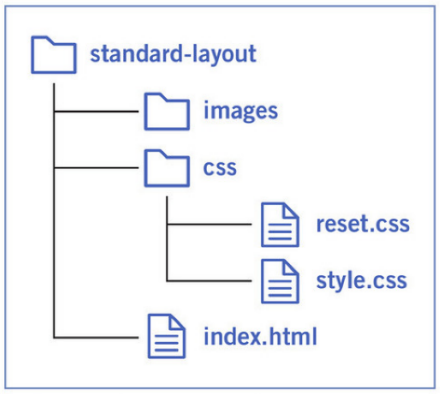
\includegraphics[width=19.00zw]{./PART2/Fig/Fig01_03.PNG}
\end{wrapfigure}
今回制作するスタンダードレイアウトサイトのファイル構成を確認しておく。
ベースになるファイルは、翔泳社のダウンロードサイト\footnote{http://www.shoeisha.co.jp/book/download/9784798141572}で配布されている。
ファイルをダウンロードしたら css/reset.css と image/ 以下のファイルはダウンロードしたファイルをそのまま利用する。\\

メインとなる index.html と css/style.css をこれから記述していく。
%%
%% 節:要素とサイズの確認
%%--------------------------------------------------------------------------------------------------------------------%%
\section{要素とサイズの確認}
